%
% Modified by Sameer Vijay
% Last Change: Wed Jul 27 2005 13:00 CEST
%
%%%%%%%%%%%%%%%%%%%%%%%%%%%%%%%%%%%%%%%%%%%%%%%%%%%%%%%%%%%%%%%%%%%%%%%%
%
% Sample Notre Dame Thesis/Dissertation
% Using Donald Peterson's ndthesis classfile
%
% Written by Jeff Squyres and Don Peterson
%
% Provided by the Information Technology Committee of
%   the Graduate Student Union
%   http://www.gsu.nd.edu/
%
% Nothing in this document is serious except the format.  :-)
%
% If you have any suggestions, comments, questions, please send e-mail
% to: ndthesis@gsu.nd.edu
%
%%%%%%%%%%%%%%%%%%%%%%%%%%%%%%%%%%%%%%%%%%%%%%%%%%%%%%%%%%%%%%%%%%%%%%%%

%
% Chapter 2
%

\chapter{Large-scale Dataset}
\label{chap:dataset}
As espoused by the MIT Reality Mining group in \cite{Nathan3,Nathan1}, the increasing availability and reliability of smartphones affords incredible opportunities for the unobtrusive gathering of data with regards to usage, location, and performance.  Although quite expensive to gather versus user self-reporting or user volunteers, a fully instrumented smartphone represents a veritable wealth of data that can afford unique insight into the smartphone performance study.

In August of 2011, two hundred participants were selected from the incoming freshmen class of our university and received a free Android smartphone and plan in exchange for agreement to participate in the two-year data collection project.  Each Android device was rooted and a custom ROM installed (Cyanogenmod) to enable the device being permanently Bluetooth discoverable. A user-level agent was installed on each of the smartphones that extracted a wide variety of environmental and usage data from the phone at periodic intervals.  The monitoring agent was installed to start automatically when the smart phone power was turned on and ran passively in the background. Tuning was conducted on the agent to ensure that even with WiFi enabled and Bluetooth always discoverable for a battery life potential at distribution of roughly one and a half days.  

\section{Data Collection}
In order to build a flexible and stable platform for delivering on-going subject queries in a secure and efficient way, we designed and implemented the monitoring system in the Fall of 2010 and did a few serials of tests before the study began. The key part of the monitoring system is the customized agent installed on the smartphones named \textit{PhoneMonitor} as illustrated in Figure~\ref{fig:agent}. The Android platform was selected for its customization capabilities through normal API or rooted/customized interfaces with respect to hardware-level interactions. It collects a variety of types of data as illustrated in table~\ref{table:data} and each kind of data is invoked through the corresponding function calls. Separate threads are employed to compensate for the variety of speeds at which the respective functions retrieve relevant data. For example, the Bluetooth data includes the detailed values of timestamp, RSSI (Received signal strength indication), MAC address, and Bluetooth identifier (BTID) with a default sensing granularity of once per minutes. The wireless environmental data (primarily WiFi) has similar fields except the access point (AP) name is recorded and the granularity of sensing is three minutes. Traffic data includes breakdowns by application and wireless adapter (cell, WiFi) with respect to both downlink (Rx) and uplink (Tx) usage at intervals down to as low as once per minute. The light sensor data, which includes the timestamp and sensor values, can help us to determine whether the phone is sheltered (e.g. inside a backpack or in hand) and the surroundings (e.g. inside or outside buildings) during the daytime. It is recorded if the current value changes more than 30 compared with the last recorded value. For mail data, both sender and receiver email addresses are recorded without content snooping. More detailed information about collected data can be found in table~\ref{table:detailed_data}. Graphic User Interface (GUI) of the application allows participants to read the last check-in time as well as the status of the network connection and Bluetooth. 

\begin{figure}[h!tbp]
\centering 
{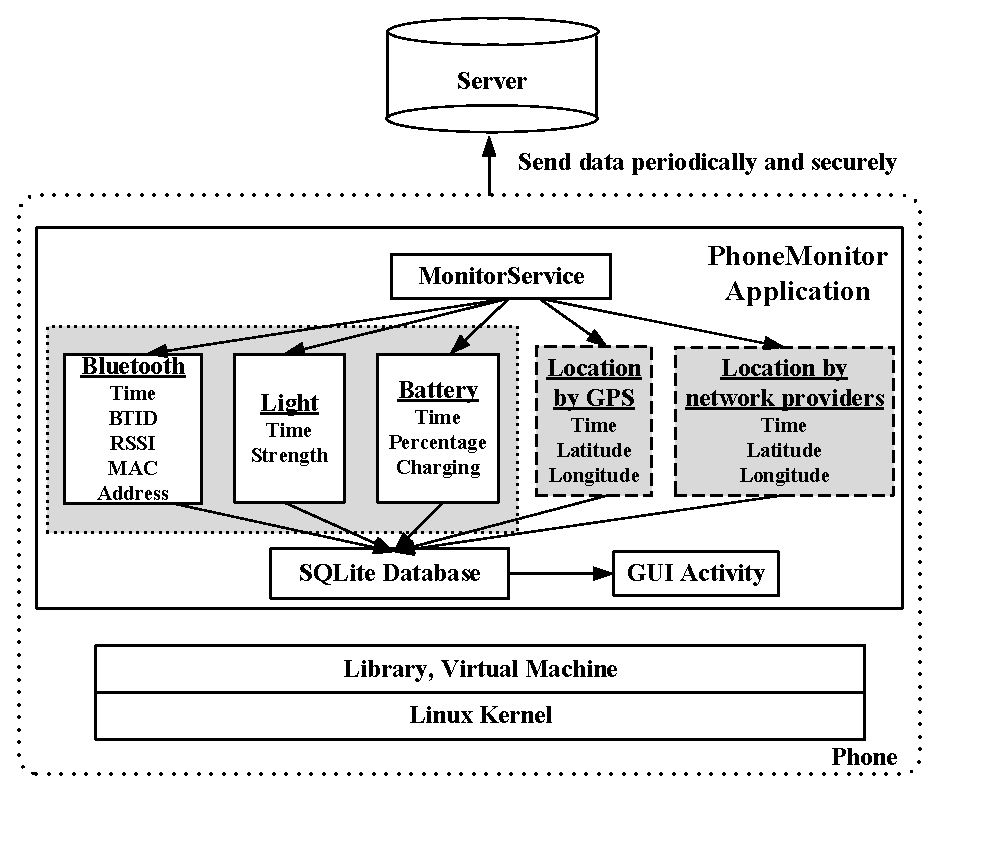
\includegraphics[width=3.5in]{graphs/Figure1.eps}}
\caption{Design of PhoneMonitor} 
\label{fig:agent}
\end{figure} 

\begin{table}[ht] 
\caption{Types of data collected in PhoneMonitor application} 
\centering  
\begin{tabular}{|l|m{10cm}|}
\hline
{\bf Device Information} & Bluetooth, WiFi, Cell, Location, Light Sensor, Screen On/Off, Battery Level, Connection Status, Network Traffic, Application Usage, Port Information, Running/Install Apps, Password, Contacts, Camera Usage\\
\hline
{\bf Digital Communication} & Phone Call, SMS, Mail, Web Browser History, Music\\
\hline
\end{tabular}
\label{table:data} 
\end{table}

Figure~\ref{fig:system} illustrates the framework of smartphone data collection, storage and query process. Data is locally spooled on the phone before being securely transmitted to one of two remote check-in servers.  Data from the check-in server is then spooled locally before being conveyed to a database server not directly connected to the Internet with all accesses strictly logged and validated to protect sensitive user data. From September 2011 to September 2013, we got more than 250G data in the database. 

\begin{figure}[h!tbp]
\centering 
{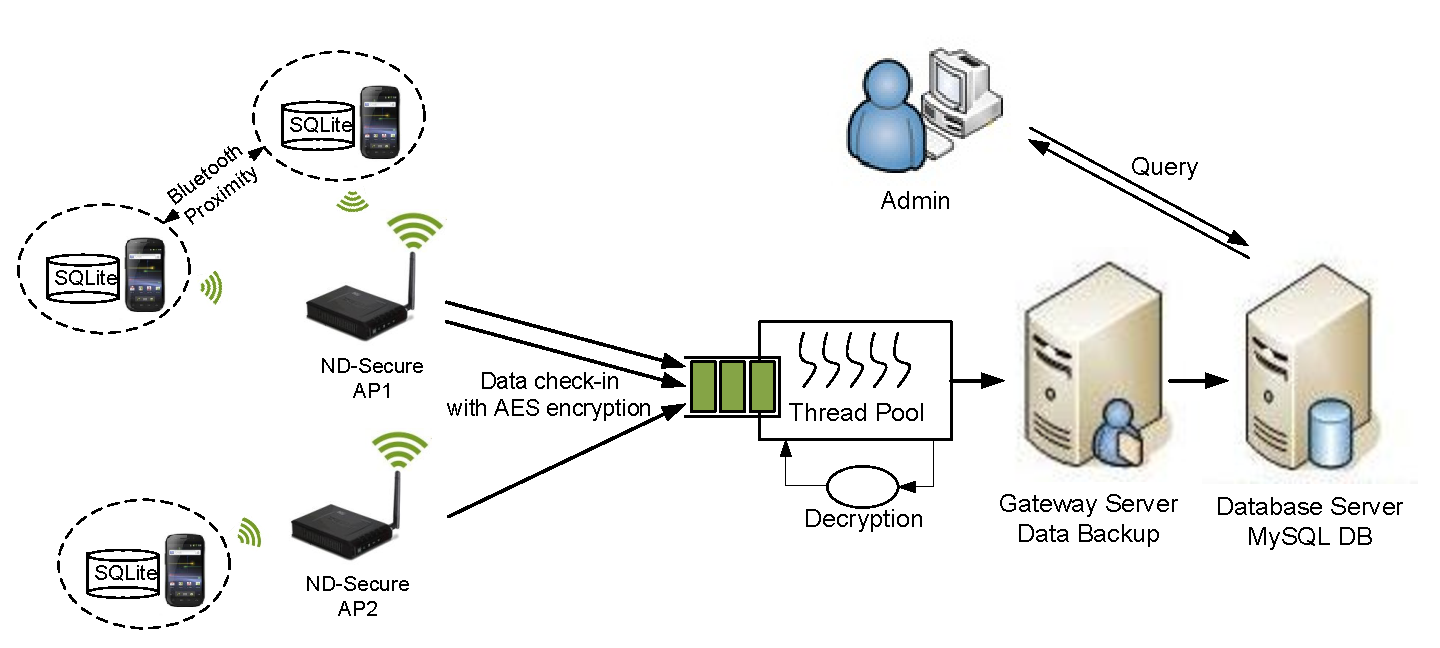
\includegraphics[width=6in]{graphs/system.eps}}
\caption{Smartphone monitoring system} 
\label{fig:system}
\end{figure} 

\section{Dataset Overview}
The dataset used in the dissertation covers 15 months data (Oct 2011 - Dec 2012) and there are around 41 million Bluetooth records, 50 million WiFi scans and 1 million SMS messages. Data from the first two months of the study is excluded to allow for the new freshmen to have settled into a new routine and social arrangements.  A reasonable degree of co-location exists amongst students in the study with students selected clustered amongst six primary dormitories equally divided amongst male and female students.  Once entered into the study, students were free to re-locate at either the beginning of the spring semester (2012) or the start of their sophomore year.  Moreover, the respective distribution levels within individual dormitories made it reasonably close to random chance amongst incoming freshmen for that dormitory if two participants in the study were selected as roommates. At the onset of the monitored period for the paper, approximately 11 students had dropped from the student reducing the data pool to 189 students.  

Table~\ref{table:summary} summarizes the details of the data across different months.  For each of the respective metrics presented in the table, we reduce the sampling rate to five minutes slots scattered throughout the day where each day has the potential for 288 measurement points.  The powered on percentage represents the number of slots when the phone monitor was active with a noticeable drop during later hours (12am - 8 am) but a notable uptick during the evening hours (4pm-12am).  The screen on percentage is the duration when the phone screen is on and implies the average usage of the phone for either consuming data or conducting other communications (SMS, phone call, etc.).  The monthly Bluetooth and WiFi records shows the average number of distinguished Bluetooth devices/WiFi APs detected per device across the month.  University virtual APs are reduced to a single AP as each university router offers between two to four WiFi AP names.  

Figure~\ref{fig:num_cdf} exhibits the empirical distribution functions (ECDF) of different types of data in April 2012 to offer additional context for the data beyond the average values denoted in Table \ref{table:summary}.  Two percentage value ECDFs are plotted (power on, screen on) together with two detected environmental values (unique Bluetooth devices in the month, unique APs in the month).  Scales for each of the two values are the lower axis for percentage and upper axis for raw numeric counts.   Most notably, the average number of unique Bluetooth devices detected in April 2012 was 746 with some devices seeing as high as over 1000 devices and others seeing as low as slightly less than 200 unique devices.  Table~\ref{table:summary} also contains distinctions with respect to intra-study proximity and inter-study breakdowns of the various Bluetooth devices.  As would be expected, intra-study detection dramatically trails off during summer break in tandem with detected university APs as the students leave campus.       

\begin{table}[tb] 
\caption{Monthly Data Summary} 
\centering
\begin{tabular}{p{6cm}|c|c|c|c}
\hline
		  Avg. Monthly Values per Phone							& Nov 2011 & Apr 2012 & Jul 2012 & Nov 2012 \\ [0.5ex] 
\hline\hline Powered On (\%) 										& 73.7 	   & 70.6 	      & 51.3 	& 61.2		\\ 
\hline	  Powered On (\%) (12am-8am) 							&  66.7	    & 60.7 		& 42.3 	& 58.0 \\
\hline 	  Powered On (\%) (8am-4pm) 								& 74.6 	   & 69.3 	      & 51.3 	& 62.7 \\
\hline 	  Powered On (\%) (4pm-12am)   			 				& 79.6	    & 72.7 		& 60.1 	& 62.9 \\
\hline	  Screen On (\%)										&  5.74	    & 5.05 		& 4.99 	& 4.30 \\
\hline	  Total Rx Traffic  (MB)									&  609.2	    & 727.2 	& 864.5 	& 685.8 \\
\hline	  Total Tx Traffic  (MB)									&  133.11	    & 123.8 	& 130.4 	& 200.8 \\
\hline 	  \# of Detected Distinct Bluetooth Devices					&  961 	     & 746 		& 310 	& 681	 \\
\hline 	  \# of Detected Distinct Bluetooth Devices Within Project (RSSI $>=$ -80dBm) 	&  131 	     & 106 		 & 	$<$1 & 75	 \\
\hline	  \# of Detected Distinct WiFi APs 										&  1218 	     & 1004	 	& 1777 	& 1663 \\
\hline	  \# of Detected Distinct WiFi APs in Campus 								&  424 	     & 446	 	& $<$1 	& 433 \\
\hline
\end{tabular}
\label{table:summary} 
\end{table}

\begin{figure}[tbp]
\centering 
{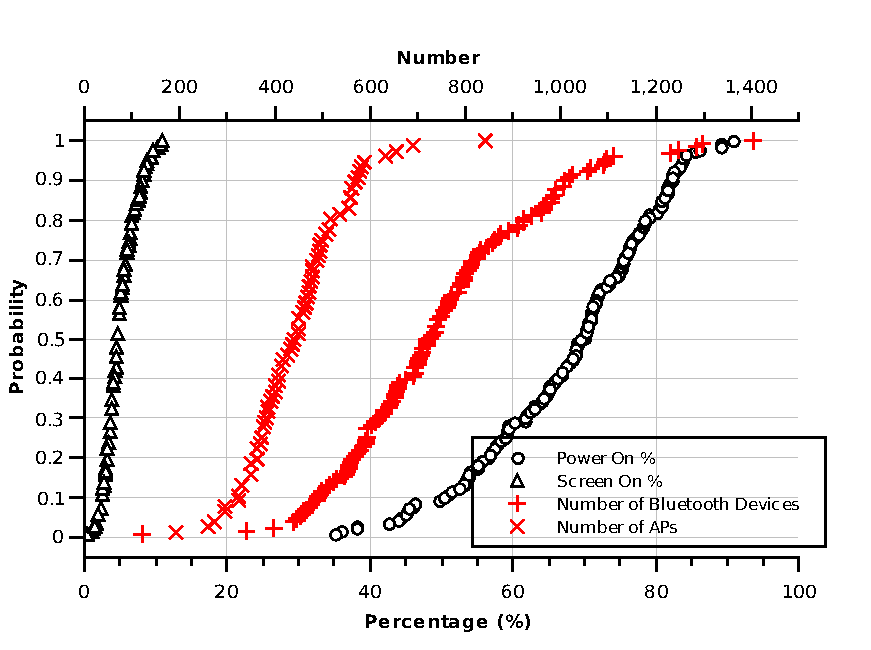
\includegraphics[width=3.5in]{graphs/num_cdf.pdf}}
\caption{ECDF of Data in April 2012} 
\label{fig:num_cdf}
\end{figure} 

\section{Comparison}
The inclusion of a device-side agent on a live user device introduces notable complexity with respect to user privacy and IRB (Institutional Review Board) concerns.  Moreover, such studies tend to be frequently expensive to conduct due to the cost of subsidizing access costs at a sufficient level to yield effective participatory compliance. Although there are several notable wireless datasets including university campuses (MIT Reality~\cite{Nathan3}, UCSD~\cite{mcnett2005access} and Dartmouth~\cite{henderson2004changing}), conference sites (Infocom~\cite{chaintreau2007impact}) and cities (Nokia~\cite{laurila2012mobile}), most datasets are limited in size and scope in terms of capturing dyadic relationships, namely both sides of a potential proximity relationship for the purposes of truly evaluating opportunistic networking.  For instance, both the MIT Reality and Infocom traces record when contact is detected by virtue of Bluetooth discovery, ample for characterizing the inter-contact times but not necessarily capturing energy levels nor traffic needs of the respective nodes.  Alternatively, the UCSD and Dartmouth traces rely on WiFi for localization gathering either data via AP fingerprinting (UCSD) or SNMP logs directly from the AP (Dartmouth).  The richest of the datasets is the data from the Nokia Data Challenge which includes both WiFi and Bluetooth data but the dataset is no longer public after the completion of the analysis.  In contrast to prior works, our dataset includes nominal proximity (Bluetooth) / location data (WiFi, Google Location service) in addition to a complete view of the smartphone environment including WiFi signal strengths, energy levels, traffic demands, and the social context for the participants in the study (Facebook, SMS, etc.).  Table~\ref{table:datasets} summarizes the most relevant studies and compares the works to our own reference study.  

\begin{landscape}
\begin{table*}[t] 
\caption{Dataset Comparison} 
\centering
\scalebox{1}{
\begin{tabular}{c|c|c|c|c|c|c}
\hline
  			Traces 				&  Our Dataset  	&  MIT Reality 	 & 	UCSD 		& Dartmouth 	& Infocom  	& Nokia \\ [0.5ex] 
\hline
\hline		Device  				& Smartphone		&  Cell Phone	 & 	PDA			& Laptop PDA & iMote		&Smartphone \\
\hline		\# of Devices 			& 189			& 97			 & 	275			& 6,648		& 41			& 185\\
\hline		Network Type 			&  Bluetooth/WiFi	& Bluetooth	 &     WiFi			& WiFi 		& Bluetooth	& Bluetooth/WiFi\\
\hline		Contact Type 			& Direct/AP-based	& Direct		 & 	AP-based		& AP-based	& Direct		& Direct/AP-based\\
\hline		Duration (days)			& 458			& 246		 & 	77			& 114		& 4			& 210\\
\hline		Granularity (seconds) 	& 60/300			& 300		 & 	120			& 300		& 120		& N/A\\
\hline		\# of internal contacts 	& 3,616,184 		& 54,667		 &	195,364		& 4,058,284	& 22,459		& N/A\\
\hline		Internal pairwise contact/day	& 0.221		& 0.022		 & 	 0.034		& 0.008		& 3.4		& N/A\\	
\hline		Other proximity related data	& Cell, Traffic, etc.	& Cell	 & 	N/A			& N/A		& N/A		& Cell, etc.\\
\hline
\end{tabular}}
\label{table:datasets} 
\end{table*}
\end{landscape}
